\documentclass[8pt,a4paper,compress,handout]{beamer}

\usepackage{/home/siyer/lib/slides}

\title{Modules and Clients}
\date{}

\begin{document}
\begin{frame}
\hfill
\begin{minipage}{150pt}
\begin{flushright}
\tiny \emph{Any fool can write code that a computer can understand. Good programmers write code that humans can understand.} 

\smallskip

- MARTIN FOWLER
\end{flushright}
\end{minipage}
\vfill
\titlepage
\end{frame}

\begin{frame}
\frametitle{Outline}
\tableofcontents
\end{frame}

\section{Using Functions in Other Programs}
\begin{frame}[fragile]
Using \emph{modular programming} we can not only divide a program into functions, but also keep them in different files.

\bigskip

We distinguish between two types of Python programs:
\begin{itemize}
\item A \emph{module} contains functions that are available for use by other programs.

\item A \emph{client} is a program that makes use of a function in a module.
\end{itemize}

\bigskip

Five steps involved in creating and using modules:
\begin{enumerate}
\item In the client, import the module.

\item In the client, qualify function calls to the module.

\item In the module, compose a test client.

\item In the module, eliminate arbitrary global code.

\item Make the module accessible to the client.
\end{enumerate}

\bigskip

Modular programming enables us to independently develop and debug functions for an application and then utilize them at any later time.

\end{frame}

\begin{frame}[fragile]
\begin{framed}
\tiny gaussian.py: Accept floats $z$, $mu$, and $sigma$ as command-line arguments. Use them to test the \lstinline{phi()} and \lstinline{Phi()} functions. Write the results to standard output.
\end{framed}

\begin{lstlisting}[language=Python]
import math
import stdio
import sys

def pdf(x, mu = 0.0, sigma = 1.0):
    x = float(x - mu) / sigma
    return math.exp(- x * x / 2.0) / math.sqrt(2.0 * math.pi) / sigma

def cdf(z, mu = 0.0, sigma = 1.0):
    z = float(z - mu) / sigma
    if z < -8.0: return 0.0
    if z > +8.0: return 1.0
    total = 0.0
    term = z
    i = 3
    while total != total + term:
        total += term
        term *= z * z / i
        i += 2
    return 0.5 + total * pdf(z)
\end{lstlisting}
\end{frame}

\begin{frame}[fragile]
\begin{lstlisting}[language=Python]
def main():
    z = float(sys.argv[1])
    mu = float(sys.argv[2])
    sigma = float(sys.argv[3])
    stdio.writeln(cdf(z, mu, sigma))

if __name__ == '__main__':
    main()
\end{lstlisting}

\begin{lstlisting}[language={}]
$ python gaussian.py 820 1019 209
0.170509668691
$ python gaussian.py 1500 1019 209
0.989316483738
$ python gaussian.py 1500 1025 231
0.980122090737
\end{lstlisting}
\end{frame}

\begin{frame}[fragile]
\begin{framed}
\tiny gaussiantable.py:  Accept a mean and standard deviation as command-line arguments. Write to standard output a table of the percentage of students scoring below certain scores on the SAT, assuming the test scores obey a Gaussian  distribution with the given mean and standard deviation.
\end{framed}

\begin{lstlisting}[language=Python]
import gaussian
import stdio
import sys

def main():
    mu = float(sys.argv[1])
    sigma = float(sys.argv[2])
    for score in range(400, 1600 + 1, 100):
        percent = gaussian.cdf(score, mu, sigma)
        stdio.writef('%4d  %.4f\n', score, percent)
 
if __name__ == '__main__':
    main()
\end{lstlisting}

\begin{lstlisting}[language={}]
$ python gaussiantable.py 1019 209
 400  0.0015
 500  0.0065
 600  0.0225
 700  0.0635
 800  0.1474
 900  0.2845
1000  0.4638
1100  0.6508
1200  0.8068
1300  0.9106
1400  0.9658
1500  0.9893
1600  0.9973
\end{lstlisting}
\end{frame}

\section{Modular Programming Abstractions}
\begin{frame}[fragile]
\emph{User-defined modules} are files that each contain a set of related functions for use by other programs.

\bigskip

We use three abstractions to manage the process of developing user-defined modules:
\begin{enumerate}
\item Application programming interfaces (APIs)
\begin{center}
\begin{tabular}{cc}
function call & description \\ \hline
\lstinline$pdf(x, mu, sigma)$ & Gaussian pdf \\
\lstinline$cdf(z, mu, sigma)$ & Gaussian cdf \\
\end{tabular} 
\end{center}

\item Clients
\begin{lstlisting}[language=Python]
percent = gaussian.cdf(score, mu, sigma)
\end{lstlisting}

\item Implementations
\begin{lstlisting}[language=Python]
def pdf(x, mu = 0.0, sigma = 1.0):
    ...
    
def cdf(z, mu = 0.0, sigma = 1.0):
    ...
\end{lstlisting}
\end{enumerate}
\end{frame}

\begin{frame}[fragile]
A \emph{library} is a collection of related modules. For example, \emph{NumPy} is a library for scientific computing.

\bigskip

A \emph{private function}, having its name start with an underscore by convention, is a helper function that is not intended to be called directly by clients. 
\begin{lstlisting}[language=Python]
def _phi(x):
    return math.exp(- x * x / 2.0) / math.sqrt(2 * math.pi)
    
def phi(x, mu = 0.0, sigma = 1.0):
    return _phi(float((x - mu) / sigma)) / sigma
\end{lstlisting}

\bigskip

Documentation for modules and their functions is provided by embedding the documentaion string in triple quotes.
\begin{lstlisting}[language=Python]
"""
stdrandom.py

The stdrandom module defines functions related to pseudo-random numbers.
"""
...
def uniformInt(lo, hi):
    """
    Return an integer chosen uniformly from the range [lo, hi).
    """
    return random.randrange(lo, hi)
...
\end{lstlisting}
\end{frame}

\section{Random Numbers}
\begin{frame}[fragile]
API for \lstinline{stdrandom} module:
\begin{center}
\begin{tabular}{cc}
function call & description \\ \hline
\lstinline$seed(i)$ & seed the random number generator with integer $i$ \\
\lstinline$uniformInt(lo, hi)$ & uniform random integer in the range $[lo, hi)$ \\
\lstinline$uniformFloat(lo, hi)$ & uniform random float in the range $[lo, hi)$ \\
\lstinline$bernoulli(p)$ & \lstinline$True$ with probability $p$ (defaults to 0.5) \\
\lstinline$binomial(n, p)$ & \makecell{number of heads in $n$ coin flips, each of which is \\ heads with probability $p$ (defaults to 0.5)} \\
\lstinline$gaussian(mu, sigma)$ &  \makecell{normal, mean $mu$ (defaults to 0), \\ standard deviation $sigma$ (defaults to 1)} \\
\lstinline$discrete(a)$ & $i$ with probability proportional to $a[i]$ \\
\lstinline$shuffle(a)$ & randomly shuffle the list $a$ \\
\lstinline$exp(lambd)$ & a float from an exponential distribution with rate $lambd$ 
\end{tabular} 
\end{center}
\end{frame}

\begin{frame}[fragile]
\begin{framed}
\tiny stdrandom\_client.py: Accept integer $trials$ as a command-line argument. Plot $trials$ number of $(x, y)$ points to standard draw, where $x$ and $y$ are drawn from a Gaussian distribution.
\end{framed}

\begin{lstlisting}[language=Python]
import stddraw
import stdrandom
import sys

trials = int(sys.argv[1])
stddraw.setPenRadius(0.0)
for i in range(trials):
    x = stdrandom.gaussian(0.5, 0.2)
    y = stdrandom.gaussian(0.5, 0.2)
    stddraw.point(x, y)
stddraw.show()
\end{lstlisting}

\begin{minipage}{160pt}
\begin{lstlisting}[language={}]
$ python stdrandom_client.py 100000
\end{lstlisting}
\end{minipage}%
\begin{minipage}{140pt}
\hfill 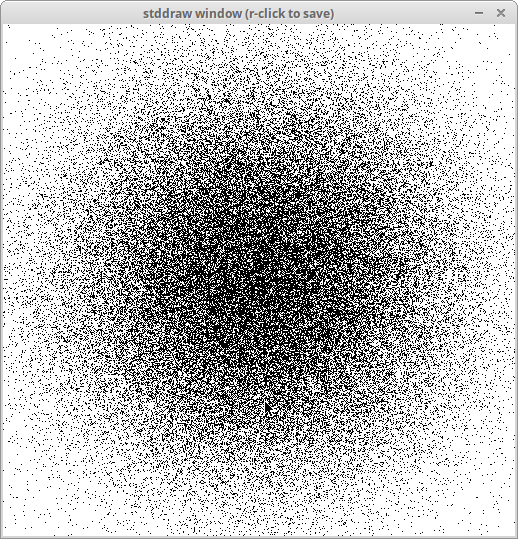
\includegraphics[scale=0.17]{figures/stdrandom_client.png}
\end{minipage}
\end{frame}

\begin{frame}[fragile]
\begin{framed}
\tiny stdrandom.py: Random number module that defines functions related to pseudo-random numbers.
\end{framed}

\begin{lstlisting}[language=Python]
import random
import math

def seed(i = None):
    random.seed(i)

def uniformInt(lo, hi):
    return random.randrange(lo, hi)
    
def uniformFloat(lo, hi):
    return random.uniform(lo, hi)

def bernoulli(p = 0.5):
    return random.random() < p

def binomial(n, p = 0.5):
    heads = 0
    for i in range(n):
        if bernoulli(p):
            heads += 1
    return heads
    
def gaussian(mean = 0.0, stddev = 1.0):
    return random.gauss(mu, sigma)
\end{lstlisting}
\end{frame}

\begin{frame}[fragile]
\begin{lstlisting}[language=Python]
def discrete(a):
    r = uniformFloat(0.0, sum(a))
    subtotal = 0.0
    for i in range(len(a)):
        subtotal += a[i]
        if subtotal > r:
            return i

def shuffle(a):
    random.shuffle(a)

def exp(lambd):
    return -math.log(1 - random.random()) / lambd
    
def _main():
    import sys
    import stdio
    seed(1)
    n = int(sys.argv[1])
    for i in range(n):
        stdio.writef(' %2d '   , uniformInt(10, 100))
        stdio.writef('%8.5f '  , uniformFloat(10.0, 99.0))
        stdio.writef('%5s '    , bernoulli())
        stdio.writef('%5s '    , binomial(100, .5))
        stdio.writef('%7.5f '  , gaussian(9.0, .2))
        stdio.writef('%2d '    , discrete([.5, .3, .1, .1]))
        stdio.writeln()

if __name__ == '__main__':
    _main()
\end{lstlisting}
\end{frame}

\section{List Processing}
\begin{frame}[fragile]
API for \lstinline{stdarray} module:
\begin{center}
\begin{tabular}{cc}
function call & description \\ \hline
\lstinline$create1D(n, val)$ & list of length $n$, each element initialized to $val$ \\
\lstinline$create2D(m, n, val)$ & $m$-by-$n$ list, each element initialized to $val$ \\
\lstinline$write1D(a)$ & write list $a$ to standard output \\
\lstinline$write2D(a)$ & write two-dimensional list $a$ to standard output \\
\lstinline$readInt1D()$ & list of integers, read from standard input \\
\lstinline$readInt2D()$ & two-dimensional list of integers, read from standard input \\
\lstinline$readFloat1D()$ & list of floats, read from standard input \\
\lstinline$readFloat2D()$ & two-dimensional list of floats, read from standard input \\
\lstinline$readBool1D()$ & list of booleans, read from standard input \\
\lstinline$readBool2D()$ & two-dimensional list of booleans, read from standard input
\end{tabular} 
\end{center}
\end{frame}

\begin{frame}[fragile]
\begin{framed}
\tiny sierpinski.py: Accept integer $n$ as a command-line argument. Play the chaos game on a triangle to produce Sierpinski triangle of $n$ points.
\end{framed}

\begin{lstlisting}[language=Python]
import stddraw
import stdrandom
import sys

def main():
    n = int(sys.argv[1])
    cx = [0.000, 1.000, 0.500]
    cy = [0.000, 0.000, 0.866]
    x = 0.0
    y = 0.0
    stddraw.setPenRadius(0.0)
    for i in range(n):
        r = stdrandom.uniformInt(0, 3)
        x = (x + cx[r]) / 2.0
        y = (y + cy[r]) / 2.0
        stddraw.point(x, y)
    stddraw.show()

if __name__ == '__main__':
    main()
\end{lstlisting}

\begin{minipage}{160pt}
\begin{lstlisting}[language={}]
$ python sierpinski.py 20000
\end{lstlisting}
\end{minipage}%
\begin{minipage}{140pt}
\hfill 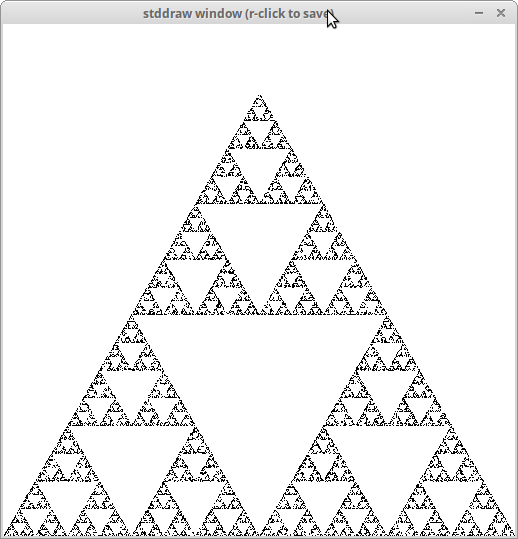
\includegraphics[scale=0.12]{figures/sierpinski.png}
\end{minipage}
\end{frame}

\begin{frame}[fragile]
\begin{framed}
\tiny ifs.py: Accept integer $n$ as a command-line argument. Read a $1$-by-$m$ vector (probabilities) and two $m$-by-$3$ matrices (coefficients for updating $x$ and $y$, respectively) from standard input. Plot the results as a set of $n$ points to standard draw.
\end{framed}

\begin{lstlisting}[language=Python]
import stdarray
import stddraw
import stdrandom
import sys

def main():
    n = int(sys.argv[1])
    dist = stdarray.readFloat1D()
    cx = stdarray.readFloat2D()
    cy = stdarray.readFloat2D()
    x = 0.0
    y = 0.0
    stddraw.setPenRadius(0.0)
    for i in range(n):
        r = stdrandom.discrete(dist)
        x0 = cx[r][0] * x + cx[r][1] * y + cx[r][2]
        y0 = cy[r][0] * x + cy[r][1] * y + cy[r][2]
        x = x0
        y = y0
        stddraw.point(x, y)
    stddraw.show()

if __name__ == '__main__':
    main()
\end{lstlisting}
\end{frame}

\begin{frame}[fragile]
Sierpinski triangle:

\begin{minipage}{160pt}
\begin{lstlisting}[language={}]
$ more sierpinski.txt
3   
  .33 .33 .34 
3 3 
  .50 .00 .00 
  .50 .00 .50 
  .50 .00 .25 
3 3 
  .00 .50 .00 
  .00 .50 .00 
  .00 .50 .433 
$ python ifs.py 20000 < sierpinski.txt
\end{lstlisting}
\end{minipage}%
\begin{minipage}{140pt}
\begin{center}
\hfill 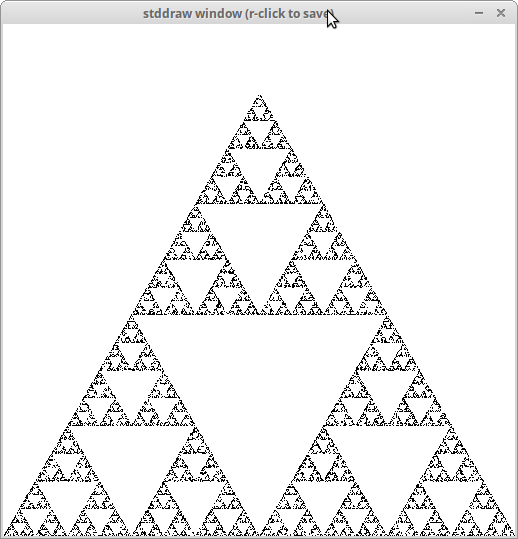
\includegraphics[scale=0.17]{figures/sierpinski.png}
\end{center}
\end{minipage}

\bigskip

Barnsley fern:

\begin{minipage}{160pt}
\begin{lstlisting}[language={}]
$ more barnsley.txt
4
   0.01  0.85  0.07  0.07
4 3
   0.00  0.00  0.500
   0.85  0.04  0.075
   0.20 -0.26  0.400
  -0.15  0.28  0.575
4 3
   0.00  0.16  0.000
  -0.04  0.85  0.180
   0.23  0.22  0.045
   0.26  0.24 -0.086
$ python ifs.py 20000 < barnsley.txt
\end{lstlisting}
\end{minipage}%
\begin{minipage}{140pt}
\begin{center}
\hfill 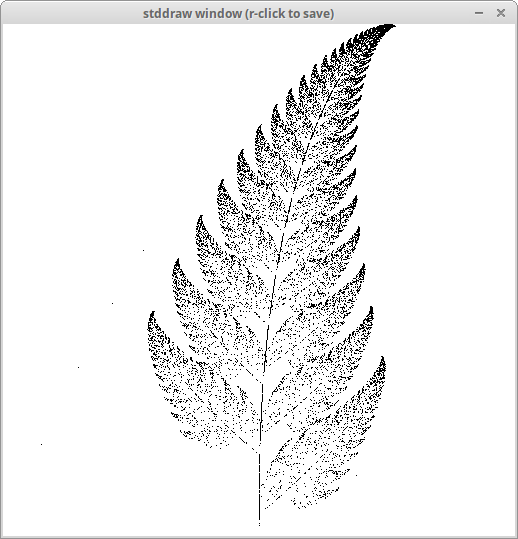
\includegraphics[scale=0.17]{figures/barnsley.png}
\end{center}
\end{minipage}
\end{frame}

\begin{frame}[fragile]
\begin{framed}
\tiny stdarray.py: List module that defines functions related to creating, reading,
and writing one- and two-dimensional lists.
\end{framed}

\begin{lstlisting}[language=Python]
import stdio

def create1D(length, value=None):
    return [value] * length

def create2D(rowCount, colCount, value=None):
    a = [None] * rowCount
    for row in range(rowCount):
        a[row] = [value] * colCount
    return a

def write1D(a):
    length = len(a)
    stdio.writeln(length)
    for i in range(length):
        element = a[i]
        if isinstance(element, bool):
            if element == True:
                stdio.write(1)
            else:
                stdio.write(0) 
        else:
            stdio.write(element)
        stdio.write(' ')
    stdio.writeln()
\end{lstlisting}
\end{frame}


\begin{frame}[fragile]
\begin{lstlisting}[language=Python]
def write2D(a):
    rowCount = len(a)
    colCount = len(a[0])
    stdio.writeln(str(rowCount) + ' ' + str(colCount))
    for row in range(rowCount):
        for col in range(colCount):
            element = a[row][col]
            if isinstance(element, bool):
                if element == True:
                    stdio.write(1)
                else:
                    stdio.write(0)
            else:
                stdio.write(element)
            stdio.write(' ')
        stdio.writeln()

def readInt1D():
    count = stdio.readInt()
    a = create1D(count, None)
    for i in range(count):
        a[i] = stdio.readInt()
    return a

def readInt2D():
    rowCount = stdio.readInt()
    colCount = stdio.readInt()
    a = create2D(rowCount, colCount, 0)
    for row in range(rowCount):
        for col in range(colCount):
            a[row][col] = stdio.readInt()
    return a
\end{lstlisting}
\end{frame}


\begin{frame}[fragile]
\begin{lstlisting}[language=Python]
def readFloat1D():
    count = stdio.readInt()
    a = create1D(count, None)
    for i in range(count):
        a[i] = stdio.readFloat()
    return a

def readFloat2D():
    rowCount = stdio.readInt()
    colCount = stdio.readInt()
    a = create2D(rowCount, colCount, 0.0)
    for row in range(rowCount):
        for col in range(colCount):
            a[row][col] = stdio.readFloat()
    return a

def readBool1D():
    count = stdio.readInt()
    a = create1D(count, None)
    for i in range(count):
        a[i] = stdio.readBool()
    return a
\end{lstlisting}
\end{frame}


\begin{frame}[fragile]
\begin{lstlisting}[language=Python]
def readBool2D():
    rowCount = stdio.readInt()
    colCount = stdio.readInt()
    a = create2D(rowCount, colCount, False)
    for row in range(rowCount):
        for col in range(colCount):
            a[row][col] = stdio.readBool()
    return a

def _main():
    write2D(readFloat2D())
    write2D(readBool2D())

if __name__ == '__main__':
    _main()
\end{lstlisting}
\end{frame}

\section{Standard Statistics}
\begin{frame}[fragile]
API for \lstinline{stdstats} module:
\begin{center}
\begin{tabular}{cc}
function call & description \\ \hline
\lstinline$mean(a)$ & average of the values in the numeric list $a$ \\
\lstinline$var(a)$ & sample variance of the values in the numeric list $a$ \\
\lstinline$stddev(a)$ & sample standard deviation of the values in the numeric list $a$ \\
\lstinline$median(a)$ & median of the values in the numeric list $a$ \\
\lstinline$plotPoints(a)$ & point plot of the values in the numeric list $a$ \\
\lstinline$plotLines(a)$ & line plot of the values in the numeric list $a$ \\
\lstinline$plotBars(a)$ & bar plot of the values in the numeric list $a$
\end{tabular} 
\end{center}
\end{frame}

\begin{frame}[fragile]
\begin{framed}
\tiny bernoulli.py: Accept integers $n$ and $trials$ as command-line arguments. Perform $trials$ experiments, each of which counts the number of heads found when a fair coin is flipped $n$ times. Then draw the results to standard draw. 
\end{framed}

\begin{lstlisting}[language=Python]
import gaussian
import math
import stdarray
import stddraw
import stdrandom
import stdstats
import sys

def main():
    n = int(sys.argv[1])
    trials = int(sys.argv[2])
    freq = stdarray.create1D(n + 1, 0)
    for t in range(trials):
        heads = stdrandom.binomial(n, 0.5)
        freq[heads] += 1
    norm = stdarray.create1D(n + 1, 0.0)
    for i in range(n + 1):
        norm[i] = 1.0 * freq[i] / trials
    phi = stdarray.create1D(n + 1, 0.0)
    stddev = math.sqrt(n) / 2.0
    for i in range(n + 1):
        phi[i] = gaussian.pdf(i, n / 2.0, stddev)
    stddraw.setCanvasSize(1000, 400)
    stddraw.setYscale(0, 1.1 * max(max(norm), max(phi)))
    stdstats.plotBars(norm)
    stdstats.plotLines(phi)
    stddraw.show()

if __name__ == '__main__':
    main()
\end{lstlisting}
\end{frame}

\begin{frame}[fragile]
\begin{minipage}{160pt}
\begin{lstlisting}[language={}]
$ python bernoulli.py 20 100000
\end{lstlisting}
\end{minipage}%
\begin{minipage}{140pt}
\hfill 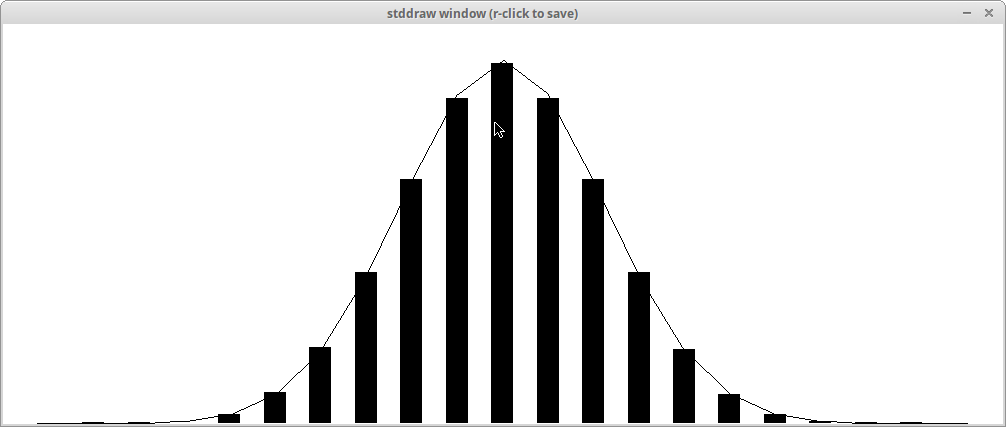
\includegraphics[scale=0.12]{figures/bernoulli.png}
\end{minipage}
\end{frame}

\begin{frame}[fragile]
\begin{framed}
\tiny stdstats.py: Statistics module that defines functions related to statistical analysis and graphical data display.
\end{framed}

\begin{lstlisting}[language=Python]
import math
import stddraw

def mean(a):
    return sum(a) / float(len(a))

def var(a):
    mu = mean(a)
    total = 0.0
    for x in a:
        total += (x - mu) * (x - mu)
    return total / (float(len(a)) - 1.0)

def stddev(a):
    return math.sqrt(var(a))

def median(a):
    b = list(a)
    b.sort()
    length = len(b)
    if length % 2 == 1:
        return b[length / /2]
    else:
        return float(b[length // 2 - 1] + b[length // 2]) / 2.0

def plotPoints(a):
    n = len(a)
    stddraw.setXscale(-1, n)
    stddraw.setPenRadius(1.0 / (3.0 * n))
    for i in range(n):
        stddraw.point(i, a[i])
\end{lstlisting}
\end{frame}

\begin{frame}[fragile]
\begin{lstlisting}[language=Python]
def plotLines(a):
    n = len(a)
    stddraw.setXscale(-1, n)
    stddraw.setPenRadius(0.0)
    for i in range(1, n):
        stddraw.line(i - 1, a[i - 1], i, a[i])

def plotBars(a):
    n = len(a)
    stddraw.setXscale(-1, n)
    for i in range(n):
        stddraw.filledRectangle(i - 0.25, 0.0, 0.5, a[i])

def _main():
    import stdarray
    import stdio
    a = stdarray.readFloat1D()
    stdio.writef('      mean %7.3f\n', mean(a))
    stdio.writef('   std dev %7.3f\n', stddev(a))
    stdio.writef('    median %7.3f\n', median(a))

if __name__ == '__main__':
    _main()
\end{lstlisting}
\end{frame}

\end{document}
